\documentclass[11pt,a4paper]{article}

\usepackage[margin=2.4cm]{geometry}
\usepackage[T1]{fontenc}
\usepackage{lmodern}
\usepackage{microtype}
\usepackage{amsmath,amssymb}
\usepackage{graphicx}
\usepackage{booktabs}
\usepackage{longtable}
\usepackage[detect-all]{siunitx}
\usepackage{xcolor}
\usepackage{listings}
\usepackage{caption}
\usepackage{tikz}
\usetikzlibrary{arrows.meta,positioning,shapes.geometric}
\usepackage[colorlinks=true,linkcolor=blue!50!black,urlcolor=blue!50!black,citecolor=blue!50!black]{hyperref}

\lstset{basicstyle=\ttfamily\small,columns=fullflexible,breaklines=true,
  frame=single,rulecolor=\color{black!25},backgroundcolor=\color{black!3},
  keepspaces=true,showstringspaces=false}

\newcommand{\code}[1]{{\ttfamily\def\_{\textunderscore\allowbreak}#1}}
\emergencystretch=2em
\newcommand{\vect}[1]{\mathbf{#1}}

\title{\textbf{Satellite Localisation with the TART Network}\\[4pt]
\large Stage 1: Common GNSS Visibility Windows for Three TART Stations\\
\normalsize Technical report --- \code{tart\_gnss} v0.1.0}
\author{Nadeem Oozeer\\ Rhodes University}
\date{7 October 2026}

\begin{document}
\maketitle

\begin{abstract}
We describe the first stage of a pipeline that will localise GNSS satellites
in three dimensions using independent all-sky images from geographically
separated Transient Array Radio Telescopes (TART). Stage~1 predicts, from
two-line element sets (TLEs) propagated with SGP4, the time intervals during
which a satellite is simultaneously above a minimum elevation (default
\ang{20}) at three selected TART stations. Window boundaries located on a
coarse time grid are refined by bisection to \SI{0.1}{\second}. For every
satellite and window the software records topocentric azimuth, elevation and
range at each station, the satellite position and velocity in the Earth-fixed
ITRS frame, line-of-sight vectors, and the full TLE provenance, so that later
stages can retrieve TART data and compare image-based direction measurements
with orbital predictions. The software is a pip-installable Python package
with a command-line interface, a test suite of 62 automated tests and
machine-readable outputs. For the Mauritius--Madagascar--South~Africa triplet
on 2026-10-01 it finds 154 common-visibility windows involving 135 of 145 GNSS
satellites.
\end{abstract}

\tableofcontents

%======================================================================
\section{Introduction}
%======================================================================

TART is a low-cost, open-source 24-element interferometer that images the
whole sky at the GPS L1 frequency (\SI{1575.42}{\mega\hertz}, bandwidth
\SI{2.5}{\mega\hertz}) \cite{tart}. Because GNSS satellites are the brightest
sources in this band, each TART image contains several satellites. Three
TART stations observing the same satellite at the same time measure three
directions; the satellite position is the point most consistent with these
lines of sight. Comparing that point with the position predicted from the
satellite's TLE provides an end-to-end test of TART imaging, calibration and
station metadata.

The full project has six steps:
\begin{enumerate}
\item identify satellites simultaneously observable by three TART stations;
\item retrieve the corresponding TART visibility observations;
\item image the satellite independently at each station;
\item estimate the satellite direction from each station;
\item infer the satellite position $(x,y,z)$ with Bayesian inference;
\item compare the inferred position with the TLE-predicted orbital position.
\end{enumerate}
This report covers \emph{only} step~1. Data retrieval, \code{tart2ms}
conversion, imaging, source extraction and inference are deliberately not
implemented, but the Stage-1 outputs are designed to drive them
(Section~\ref{sec:future}).

%======================================================================
\section{Problem definition}
%======================================================================

For satellite $s$, station $i$ and UTC time $t$, let $E_{s,i}(t)$ be the
geometric (unrefracted) topocentric elevation above the WGS84 local
horizontal. Satellite $s$ is visible from station $i$ when
\begin{equation}
E_{s,i}(t) \ge E_{\min}, \qquad E_{\min} = \ang{20}\ \text{(default)}.
\end{equation}
For a set of stations $\mathcal{S}$ (three in Stage~1) simultaneous
visibility is
\begin{equation}
V_s(t) = \bigwedge_{i\in\mathcal{S}} \bigl[E_{s,i}(t)\ge E_{\min}\bigr]
\;\Longleftrightarrow\; \min_{i\in\mathcal{S}} E_{s,i}(t) \ge E_{\min}.
\label{eq:common}
\end{equation}
A \emph{common visibility window} is a maximal continuous interval
$[t_{\rm start},t_{\rm end}]$ on which $V_s(t)$ is true, with duration
$T_{\rm common}=t_{\rm end}-t_{\rm start}$. Every window is kept as a separate
record (a satellite may have several per day), and the primary result is the
list of satellite/window pairs ranked by decreasing $T_{\rm common}$.

%======================================================================
\section{Input data and provenance}
%======================================================================

\subsection{Station coordinates}

Station coordinates are never written into the code. They are read from a
YAML (or JSON) configuration file, \code{config/stations.yaml}, in which each
entry records the WGS84 geodetic latitude, longitude and height, the TART
telescope identifier, its REST API URL, and the provenance of the
coordinates. No coordinate was estimated or invented: the values were taken
from the TART network-monitor registry
(\url{https://map.elec.ac.nz/api/v1/telescopes}, field
\code{telescopeInfo.info.location}), which mirrors each telescope's own
\code{/api/v1/info} endpoint. For \code{za-rhodes} the values were
independently confirmed from
\url{https://api.elec.ac.nz/tart/za-rhodes/api/v1/info}. All were retrieved
on 2026-10-07 at 10:03~UTC. Table~\ref{tab:stations} lists the three
stations used in this report; the configuration also contains four other
African TART stations (Hammanskraal, Namibia, Zambia, Ghana), and further
stations can be added without code changes.

\begin{table}[h]
\centering
\caption{Stations of the Stage-1 triplet. Coordinates as published by TART
(WGS84; height datum undocumented by the source). ITRS vectors computed by
Skyfield.}
\label{tab:stations}
\small
\begin{tabular}{llrrrr}
\toprule
ID & TART id & Lat.\ (deg) & Lon.\ (deg) & Alt.\ (m) & ITRS $(x,y,z)$ (km)\\
\midrule
\code{mauritius}    & \code{mu-udm}    & $-20.2587508$ & $57.7591989$ & 20.00   & (3193.40, 5063.04, $-2194.60$)\\
\code{madagascar}   & \code{mg-tana}   & $-18.8971446$ & $47.5551677$ & 1280.00 & (4074.72, 4455.38, $-2053.00$)\\
\code{south\_africa} & \code{za-rhodes} & $-33.319413$  & $26.507688$  & 642.26  & (4774.72, 2381.39, $-3483.97$)\\
\bottomrule
\end{tabular}
\end{table}

Two caveats apply. (i) These are the coordinates configured on each
telescope by its operators; their survey accuracy is not documented. An
error of a few metres is irrelevant for visibility prediction but will matter
for the Stage-5 inference, where surveyed antenna-array centres should be
used. (ii) The identifier \code{south\_africa} denotes the Rhodes University
telescope; South Africa also hosts \code{za-hammanskraal}, available as
\code{south\_africa\_hammanskraal}. Configuration loading validates each
coordinate (latitude in $[-90,90]$, longitude in $[-180,180]$, height in
$[-500,9000]$\,m, finite, non-null) and requires a non-empty \code{source}.

\subsection{Satellite catalogue}

Orbits are described by TLEs. When no catalogue is supplied the software
downloads the CelesTrak GP groups \code{gps-ops}, \code{galileo},
\code{beidou} and \code{glo-ops} \cite{celestrak}. The combined file is
archived as \code{data/tle/gnss\_<retrieval time>.tle}, never overwritten,
together with a sidecar \code{.meta.json} that records the source URLs, the
retrieval time, the SHA-256 hash of the file and the constellation of each
NORAD ID (taken from the CelesTrak group, not guessed from the name). On
reload, a SHA-256 mismatch between file and sidecar is a hard error. When a
user-supplied file has no sidecar, constellations are inferred from
satellite names with conservative patterns (\code{COSMOS} names are labelled
GLONASS only in the CelesTrak \code{COSMOS~nnnn~(slot)} form); unmatched
satellites are labelled \code{UNKNOWN} and reported. Every TLE line is checked
for length, modulo-10 checksum and NORAD-ID consistency.

For each satellite the software keeps the constellation, name, NORAD ID, TLE
lines and epoch, and for each window the signed TLE age
$\Delta t_{\rm TLE}=t_{\rm obs}-t_{\rm epoch}$ at the window start, middle
and end (negative values mean the elements are propagated backwards).

\subsection{TLE age diagnostics}

SGP4 accuracy degrades with $|\Delta t_{\rm TLE}|$, at a rate that depends on
the orbit and on the quality of the element set; there is no universal
threshold. The software therefore (a) stores $\Delta t_{\rm TLE}$ for every
window, (b) warns whenever any epoch of the search interval precedes the TLE
epoch --- the typical symptom of using a modern catalogue to reconstruct an
older observation --- and (c) warns when $|\Delta t_{\rm TLE}|$ exceeds a
user-configurable flag level (\code{--tle-age-warning-days}, default 3~days).
The flag level is a project convention, not an accuracy bound. For
historical observations, a catalogue contemporaneous with the observation
(for instance from Space-Track) should be supplied with \code{--tle-file}.

%======================================================================
\section{Method}
%======================================================================

\subsection{Time}

All times are UTC. Command-line times are ISO-8601; an explicit \code{Z} or
offset is honoured and converted to UTC, and a timezone-naive value is, by
documented convention, interpreted as UTC (and logged as such). Internally,
sample epochs are elapsed SI seconds from the start time, added on the TT
scale by Skyfield, so leap seconds are handled correctly. Skyfield's
built-in leap-second and $\Delta T$ tables are used so that runs need no
network access beyond the TLE download and are reproducible for a given
Skyfield version.

\subsection{Orbit propagation and topocentric geometry}

Propagation uses the SGP4 implementation of the \code{sgp4} package through
Skyfield \cite{skyfield,sgp4,vallado2006}; no orbital mechanics or frame
transformation is implemented by hand. For a station at geodetic position
$(\phi_i,\lambda_i,h_i)$ the vector difference
\code{(satellite - station).at(t)} gives the geometric topocentric position,
from which Skyfield returns azimuth $A_i$ (from north through east),
elevation $E_i$, range $\rho_i$ and range rate $\dot\rho_i$. Light-time,
aberration and refraction are not applied: the quantities describe geometric
lines of sight, which is what the Stage-5 forward model needs. (At
$E=\ang{20}$ tropospheric refraction raises the apparent elevation by about
$\ang{;2.7;}$, irrelevant to visibility but to be considered when comparing with
measured TART directions.)

\subsection{Earth-fixed satellite positions}

For each window the satellite position $\vect r_s$ and velocity are computed
at the start, midpoint and end in the International Terrestrial Reference
System (ITRS) using Skyfield's \code{frame\_xyz\_and\_velocity(itrs)}, which
converts SGP4's TEME output via the Earth's rotation, precession and
nutation. Skyfield's ITRS neglects polar motion unless polar-motion tables
are loaded, an approximation at the $\sim$\SI{10}{\metre} level. The
station positions $\vect r_i$ are expressed in the same frame from their
WGS84 coordinates. The geometric line of sight and its unit vector,
\begin{equation}
\vect d_i = \vect r_s - \vect r_i, \qquad
\hat{\vect d}_i = \vect d_i / \lVert \vect d_i \rVert ,
\end{equation}
are stored at the window midpoint for every station. All Cartesian outputs
carry the label \code{coordinate\_frame = "ITRS"}.

\subsection{Coarse sampling and boundary refinement}

Each satellite is propagated on a uniform grid with step $\Delta$
(default \SI{10}{\second}) that always includes both ends of the interval.
The boolean series $V_s(t_k)$ of Eq.~\eqref{eq:common} is split into maximal
runs of \code{True}. A run starting at sample $k$ brackets a rise between
$t_{k-1}$ (false) and $t_k$ (true); this bracket is refined by bisection on
the exact predicate $V_s(t)$ until it is narrower than a tolerance $\tau$
(default \SI{0.1}{\second}, i.e.\ $\lceil\log_2(\Delta/\tau)\rceil = 7$
iterations). The reported boundary is the \code{True}-side end of the final
bracket, so it is always inside the original bracket, satisfies $V_s=$ true,
and is within $\tau$ of the true crossing. Setting boundaries are treated
symmetrically. Runs touching the edges of the search interval are not
refined and are flagged as \emph{clipped} (the real window may be longer).

Because the predicate is the minimum elevation over stations, the window
boundaries are determined by whichever station is limiting at that moment;
in the results the limiting station shows $E=\ang{20.0000}$ at the boundary
(Section~\ref{sec:verification}). The only geometric limitation of the
approach is that excursions shorter than $\Delta$ (a satellite briefly
dipping below or rising above the threshold between two samples) cannot be
detected; for GNSS orbits, whose elevations change by roughly a tenth of
a degree or less per \SI{10}{\second}, this is not a practical concern, and $\Delta$
can be reduced if needed.

\subsection{Ranking}

Windows shorter than \code{--min-duration} are discarded. The remainder are
sorted by decreasing duration, ties broken by start time and then NORAD ID,
giving a deterministic 1-based rank.

%======================================================================
\section{Software}
%======================================================================

\subsection{Architecture}

The package \code{tart\_gnss} (Python $\ge 3.9$; dependencies NumPy,
Skyfield, sgp4, PyYAML) is organised as in Table~\ref{tab:modules} and
Fig.~\ref{fig:flow}. Visibility and window logic operate on a sequence of
stations of any length; only the CLI enforces the Stage-1 requirement of
exactly three stations. Network access is confined to the TLE module.
Diagnostics use Python's \code{logging} with UTC timestamps; only the final
summary is printed.

\begin{table}[h]
\centering
\caption{Package modules.}
\label{tab:modules}
\small
\begin{tabular}{lp{11cm}}
\toprule
Module & Responsibility\\
\midrule
\code{stations.py} & load YAML/JSON configuration; validate coordinates; resolve identifiers (case-insensitive, TART ids accepted)\\
\code{tle.py} & parse and checksum TLEs; epochs; constellation labels; CelesTrak download and archival with SHA-256 sidecar\\
\code{propagation.py} & SGP4 via Skyfield; azimuth, elevation, range, range rate; ITRS positions; line-of-sight vectors\\
\code{visibility.py} & $E_i\ge E_{\min}$ per station and the AND over $N$ stations; exact predicate for refinement\\
\code{windows.py} & runs of \code{True}; bisection refinement; \code{Window} objects with clipping flags\\
\code{search.py} & orchestration over satellites; window characterisation; TLE-age diagnostics\\
\code{output.py} & ranking; CSV; detailed JSON; terminal summary\\
\code{provenance.py} & software versions, hashes and run metadata\\
\code{cli.py} & argument parsing, validation, logging, file naming\\
\bottomrule
\end{tabular}
\end{table}

\begin{figure}[h]
\centering
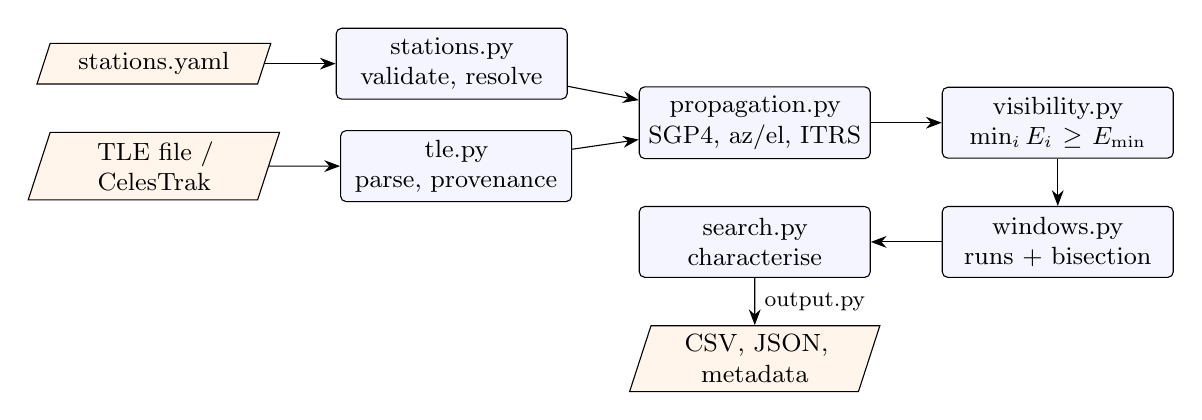
\begin{tikzpicture}[node distance=6mm and 9mm,
  box/.style={draw,rounded corners=2pt,fill=blue!4,align=center,font=\small,minimum height=9mm,text width=27mm},
  io/.style={draw,trapezium,trapezium left angle=72,trapezium right angle=108,fill=orange!8,align=center,font=\small,text width=24mm},
  >={Stealth[length=2mm]}]
\node[io] (st) {stations.yaml};
\node[io, below=of st] (tle) {TLE file /\\CelesTrak};
\node[box, right=of st] (ld) {stations.py\\validate, resolve};
\node[box, right=of tle] (tl) {tle.py\\parse, provenance};
\node[box, right=of ld, yshift=-7.5mm] (pr) {propagation.py\\SGP4, az/el, ITRS};
\node[box, right=of pr] (vi) {visibility.py\\$\min_i E_i \ge E_{\min}$};
\node[box, below=of vi] (wi) {windows.py\\runs + bisection};
\node[box, left=of wi] (se) {search.py\\characterise};
\node[io, below=of se] (out) {CSV, JSON,\\metadata};
\draw[->] (st) -- (ld); \draw[->] (tle) -- (tl);
\draw[->] (ld) -- (pr); \draw[->] (tl) -- (pr);
\draw[->] (pr) -- (vi); \draw[->] (vi) -- (wi);
\draw[->] (wi) -- (se); \draw[->] (se) -- node[right,font=\footnotesize]{output.py} (out);
\end{tikzpicture}
\caption{Data flow of a Stage-1 run.}
\label{fig:flow}
\end{figure}

\subsection{Installation and use}

\begin{lstlisting}
pip install .                      # or: pip install -e ".[dev]"
common-gnss --stations mauritius madagascar south_africa \
    --start 2026-10-01T00:00:00Z --end 2026-10-02T00:00:00Z \
    --min-elevation 20 --step 10
\end{lstlisting}
\code{python common\_gnss.py} and \code{python -m tart\_gnss} are equivalent.
Optional arguments: \code{--tle-file} (use an archived catalogue exactly),
\code{--tle-dir}, \code{--constellations GPS Galileo \dots},
\code{--output}, \code{--station-file}, \code{--min-duration},
\code{--tolerance}, \code{--tle-age-warning-days}, \code{--verbose}. Input
errors (unknown station, malformed date, start not before end, wrong number
of stations) terminate with exit status~2 and a clear message.

\subsection{Outputs}

A run writes three files (default \code{results/\allowbreak common\_gnss\_YYYYMMDD.csv},
\code{.json} and \code{run\_metadata\_YYYYMMDD.json}):
\begin{description}
\item[CSV] one row per satellite$\times$window: rank, satellite, NORAD ID,
constellation, start/end (UTC), duration, clipping flags, threshold; for each
station its identifier and azimuth/elevation at start, middle and end plus
the mid-window range; midpoint ITRS satellite position with the frame name;
TLE epoch, TLE age at start and middle, TLE source. TLE lines are not
embedded in the CSV.
\item[JSON] run parameters; frame description; stations with ITRS vectors
and sources; catalogue provenance; every searched satellite with full TLE;
and for every window the station geometry (azimuth, elevation, range, range
rate) at start/mid/end, satellite ITRS position and velocity at the same
epochs, midpoint line-of-sight vectors, and the TLE lines, epoch and ages.
\item[Metadata] versions of \code{tart\_gnss}, Python, Skyfield, sgp4, NumPy
and PyYAML; platform; run timestamp; full command line; interval;
stations and coordinates; SHA-256 of the station file; threshold, step and
tolerance; TLE file, source, retrieval time and SHA-256; TLE-age summary;
failed propagations; output paths.
\end{description}

%======================================================================
\section{Verification}
\label{sec:verification}
%======================================================================

The test suite (\code{pytest}, 62 tests, $<\SI{1}{\second}$) covers:
\begin{itemize}
\item \textbf{Stations:} latitude \ang{100}, longitude \ang{300}, implausible
heights, \code{null} or non-numeric coordinates and missing provenance are
rejected; unknown and duplicated stations fail with clear messages; the
bundled configuration validates and is sourced.
\item \textbf{TLEs:} checksum, two- and three-line parsing, epoch decoding,
name classification, constellation filtering, archival with sidecar
metadata (network mocked) and detection of a modified catalogue.
\item \textbf{Visibility:} the synthetic example
$A=[19,21,25,18]$, $B=[22,23,24,25]$, $C=[30,30,19,30]$ with $E_{\min}=\ang{20}$
gives $[\text{F},\text{T},\text{F},\text{F}]$; the threshold is inclusive;
NaN (failed propagation) is not visible; any number of stations works.
\item \textbf{Windows:} \code{F F T T T F} gives one window;
\code{F T T F F T T F} gives two independent windows; refined crossings lie
inside the coarse bracket and within tolerance of an analytic crossing;
clipping flags are set at interval edges.
\item \textbf{Propagation:} orbital radii of real GPS, Galileo, BeiDou-GEO and
GLONASS TLEs match their nominal values; geostationary elevation is nearly
constant; and the Skyfield azimuth/elevation agree to better than
\ang{0.001} with an independent east-north-up projection of the ITRS line of
sight $\vect r_s-\vect r_i$, confirming that the angular and Cartesian outputs
are mutually consistent --- a prerequisite for the Stage-5 forward model.
\item \textbf{CLI:} start after end, malformed dates, unknown stations and
wrong station counts fail clearly; an end-to-end run checks ranking order,
frame labels, TLE lines in the JSON, that every station is above
\ang{20} at window start, middle and end, and that refined boundaries are at
\ang{20} to within \ang{0.01}; a geometry without common visibility reports
``No common GNSS visibility windows found.''
\end{itemize}
In the production run below the limiting station at every refined boundary
has $E=\ang{20.0000}$ (e.g.\ Rhodes at both boundaries of the BeiDou-2~G6
window), and the ITRS radii are \SI{42146}{\kilo\metre} for GEO and
\SI{29594}{\kilo\metre} for Galileo, as expected.

%======================================================================
\section{Results: Mauritius--Madagascar--South Africa, 2026-10-01}
%======================================================================

The acceptance run covered 2026-10-01T00:00Z--2026-10-02T00:00Z with
$E_{\min}=\ang{20}$ and $\Delta=\SI{10}{\second}$, using the CelesTrak
catalogue retrieved 2026-10-07T10:11:56Z (145 satellites: 32 GPS, 32
Galileo, 54 BeiDou, 27 GLONASS; SHA-256 \code{1a6c259b\dots f2ea}). The run
took about \SI{6}{\second} of computation (excluding download).

\paragraph{TLE age.} Because the catalogue was retrieved six days after the
observation date, 127 of the 145 satellites have TLE epochs after the start
of the interval and are propagated backwards; the median $|\Delta t_{\rm TLE}|$
is 5.4~days and the maximum 18.3~days. The software warned accordingly. For
window prediction this is adequate, but the results should be regenerated
with a contemporaneous catalogue before they are used as a reference for
Stage~6.

\paragraph{Windows.} 154 common windows were found, involving 135
satellites (Table~\ref{tab:constellations}). Common windows are long because
the three stations are within $\sim$\SI{3200}{\kilo\metre} of each other while
the satellites are at altitudes of 19\,000--36\,000~km. The ten longest are
listed in Table~\ref{tab:top}; the top two are geostationary BeiDou
satellites visible for most or all of the day, so their windows are clipped
by the search interval. Figure~\ref{fig:timeline} shows the forty longest
windows, Fig.~\ref{fig:elevation} the elevation curves of the top-ranked
satellite of each constellation, and Fig.~\ref{fig:sky} the sky tracks of
the top-ranked Galileo satellite as seen from the three stations.

\begin{table}[h]
\centering
\caption{Common windows per constellation (2026-10-01).}
\label{tab:constellations}
\small
\begin{tabular}{lrrrr}
\toprule
Constellation & Satellites searched & Windows & Longest (min) & Median (min)\\
\midrule
GPS     & 32 & 37 & 320.2  & 207.4\\
Galileo & 32 & 32 & 438.2  & 265.7\\
BeiDou  & 54 & 51 & 1440.0$^\ast$ & 267.6\\
GLONASS & 27 & 34 & 264.6  & 188.6\\
\bottomrule
\multicolumn{5}{l}{\footnotesize $^\ast$ geostationary, clipped by the 24-h search interval}
\end{tabular}
\end{table}

\begin{table}[h]
\centering
\caption{Ten longest common windows (UTC, 2026-10-01; $^\ast$ clipped).
$\Delta t_{\rm TLE}$ at window middle.}
\label{tab:top}
\small
\begin{tabular}{rllllrr}
\toprule
Rank & Satellite & NORAD & Start & End & Dur.\ (min) & $\Delta t_{\rm TLE}$ (d)\\
\midrule
1 & BEIDOU-2 G5 (C05)       & 38091 & 00:00:00$^\ast$ & 24:00:00$^\ast$ & 1440.0 & $-5.48$\\
2 & BEIDOU-3 G2 (C60)       & 45344 & 04:07:05 & 24:00:00$^\ast$ & 1192.9 & $-5.39$\\
3 & BEIDOU-2 G6 (C02)       & 38953 & 12:28:02 & 20:16:28 & 468.4 & $-5.29$\\
4 & GSAT0219 (GALILEO 23)   & 43566 & 08:28:07 & 15:46:19 & 438.2 & $-4.86$\\
5 & GSAT0218 (GALILEO 22)   & 43058 & 00:00:00$^\ast$ & 07:11:58 & 432.0 & $-2.53$\\
6 & GSAT0208 (GALILEO 11)   & 41175 & 16:53:47 & 24:00:00$^\ast$ & 426.2 & $-4.27$\\
7 & GSAT0234 (GALILEO 34)   & 67162 & 15:21:34 & 22:24:29 & 422.9 & $-0.78$\\
8 & BEIDOU-2 IGSO-4 (C09)   & 37763 & 16:48:56 & 23:37:48 & 408.9 & $-2.96$\\
9 & GSAT0204 (GALILEO 8)    & 40545 & 07:08:50 & 13:51:50 & 403.0 & $15.64$\\
10 & BEIDOU-3S IGSO-1S (C31) & 40549 & 01:38:59 & 08:08:02 & 389.1 & $-2.80$\\
\bottomrule
\end{tabular}
\end{table}

\begin{figure}[p]
\centering
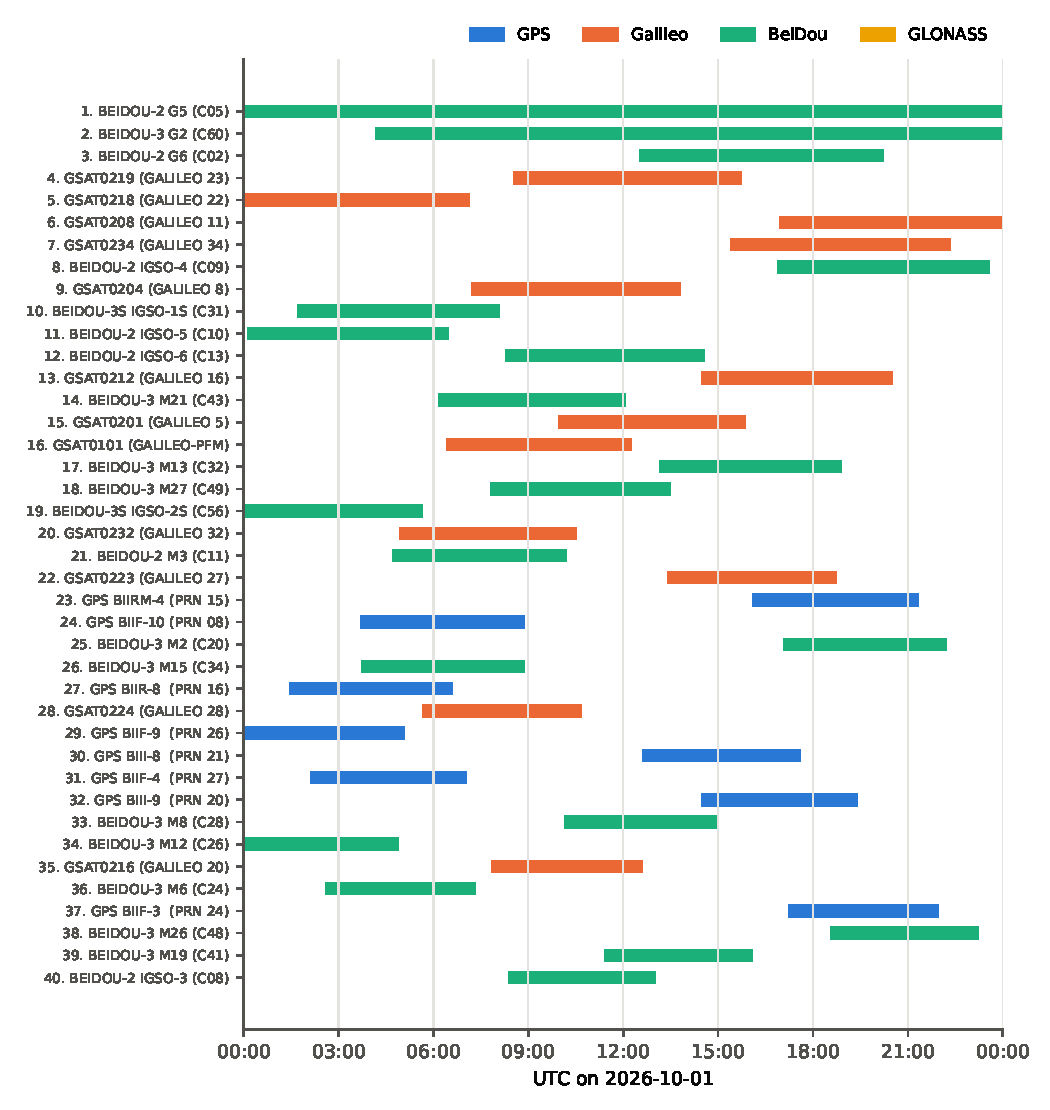
\includegraphics[width=\textwidth]{figures/window_timeline.pdf}
\caption{The forty longest common windows for the Mauritius--Madagascar--South
Africa triplet on 2026-10-01, ordered by rank and coloured by constellation.
Separate windows of the same satellite are separate rows.}
\label{fig:timeline}
\end{figure}

\begin{figure}[p]
\centering
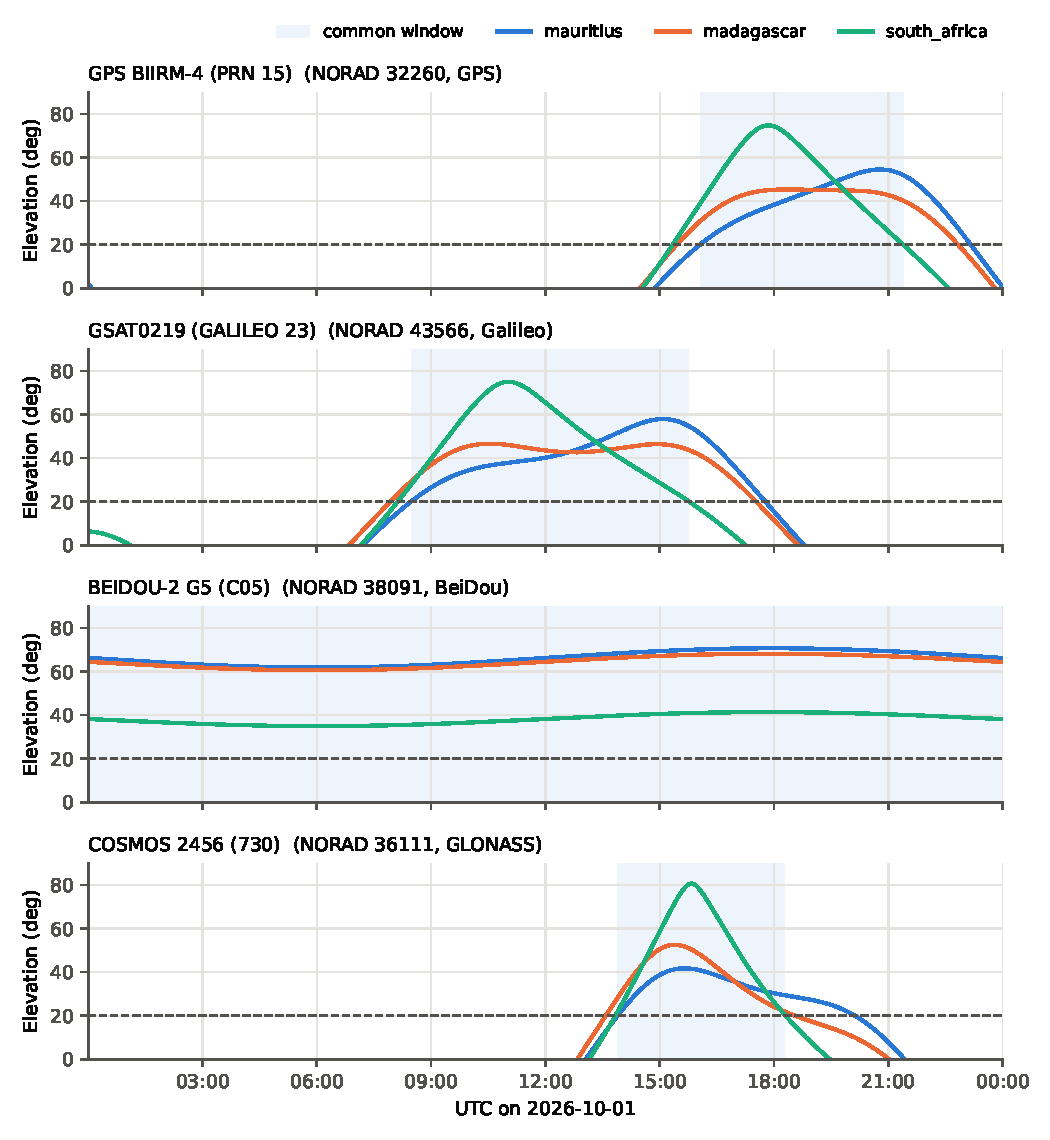
\includegraphics[width=\textwidth]{figures/elevation_examples.pdf}
\caption{Elevation at the three stations for the top-ranked window of each
constellation. The dashed line is $E_{\min}=\ang{20}$; shading marks the
common window, bounded by whichever station is limiting.}
\label{fig:elevation}
\end{figure}

\begin{figure}[h]
\centering
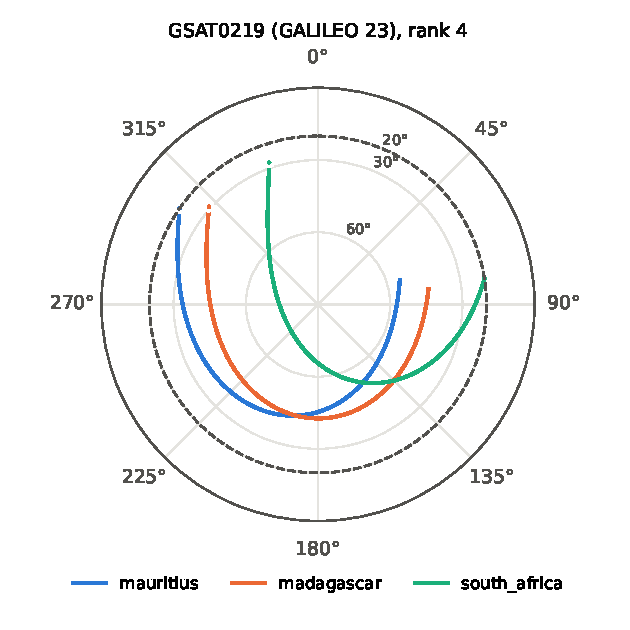
\includegraphics[width=0.55\textwidth]{figures/skyplot.pdf}
\caption{Sky tracks (azimuth clockwise from north, zenith at the centre) of
GSAT0219 during its common window, as seen from each station; dots mark the
window start and the dashed circle the \ang{20} horizon. These are the
directions that TART images will measure in Stages~3--4.}
\label{fig:sky}
\end{figure}

\paragraph{Relevance at 1.575 GHz.} Stage~1 is purely geometric, and
geometric visibility does not imply detectability by TART, which records
\SI{2.5}{\mega\hertz} around \SI{1575.42}{\mega\hertz}. GPS L1, Galileo E1
and BeiDou-3 B1C share this centre frequency, whereas BeiDou-2 transmits B1I
at \SI{1561.098}{\mega\hertz} and the legacy GLONASS L1 FDMA signals lie at
\SIrange{1598}{1606}{\mega\hertz} \cite{gnssbook}. Several of the
top-ranked windows (BeiDou-2 G5, G6, IGSO-4) are therefore unlikely to be
usable. Until signal-level filtering is added, Stage~2 should be driven by
\code{--constellations GPS Galileo} or by BeiDou-3 windows.

%======================================================================
\section{Interface to later stages}
\label{sec:future}
%======================================================================

\paragraph{Stage 2 (data retrieval).} The CSV rank identifies a window; the
JSON gives its exact UTC limits and, for each station, the TART identifier
and API URL (\code{https://api.elec.ac.nz/tart/<id>}, the pattern used by
\code{tart2ms}). A future \code{retrieve\_tart.py --visibility-results
common\_gnss.csv --rank 1} can query the three archives and reuse the
\code{tart2ms} archive and HDF5-to-Measurement-Set tooling rather than
reimplementing it. At retrieval time only the \code{za-rhodes} and
\code{ghana} APIs answered; the others must be checked before Stage~2.

\paragraph{Stage 5 (inference).} For a candidate satellite position
$\vect r_s$ in ITRS, the predicted direction at station $i$ is
$\hat{\vect d}_i(\vect r_s)$, converted to $(A_i,E_i)$ in the local
east-north-up frame. Given TART-measured directions
$(A_i^{\rm obs},E_i^{\rm obs})$ with uncertainties $\sigma_i$, a natural
likelihood is
\begin{equation}
\ln\mathcal L(\vect r_s) = -\frac12\sum_{i=1}^{3}
\frac{\theta_i^2(\vect r_s)}{\sigma_i^2} + \text{const},\qquad
\cos\theta_i = \hat{\vect d}_i(\vect r_s)\cdot\hat{\vect u}_i^{\rm obs},
\end{equation}
where $\theta_i$ is the angle between predicted and observed unit vectors.
Stage~1 already provides every ingredient of the forward model --- exact
station ITRS vectors, exact UTC epochs, TLE provenance, predicted
$(A_i,E_i)$, predicted $\vect r_s$ and line-of-sight unit vectors --- and the
verification of Section~\ref{sec:verification} shows the angular and
Cartesian predictions are consistent to better than \ang{0.001}. A
TLE-based prior on $\vect r_s$ (or its comparison in Stage~6) should account
for the TLE age recorded with each window.

%======================================================================
\section{Limitations}
%======================================================================

\begin{itemize}
\item TLE/SGP4 accuracy depends on TLE age and quality; current CelesTrak
data are not suitable for reconstructing old observations
(Sections~3.3 and~7).
\item Visibility uses geometric elevation; refraction, local horizon masks
and antenna patterns are not modelled.
\item ITRS positions neglect polar motion ($\sim$\SI{10}{\metre}).
\item Station coordinates are as published by TART, with undocumented
accuracy and height datum.
\item Excursions shorter than the coarse step are not detected.
\item The satellite list is not filtered by transmitted signal.
\end{itemize}

%======================================================================
\section{Reproducibility}
%======================================================================

A run is fully reproducible from its metadata file: the archived TLE file
(verified by SHA-256), the station file (also hashed), the software versions
and the full command line. Re-running with
\code{--tle-file data/tle/gnss\_2026-10-07T101156Z.tle} reproduces the
results in this report. Historical catalogues are never overwritten.

\begin{thebibliography}{9}
\bibitem{tart} T.~Molteno et al., \emph{TART: The Transient Array Radio
Telescope}, \url{https://tart.elec.ac.nz}; source code
\url{https://github.com/tart-telescope}.
\bibitem{celestrak} T.~S.~Kelso, \emph{CelesTrak GP element sets},
\url{https://celestrak.org/NORAD/elements/}.
\bibitem{skyfield} B.~Rhodes, \emph{Skyfield: High precision research-grade
positions for planets and Earth satellites generator}, Astrophysics Source
Code Library ascl:1907.024 (2019), \url{https://rhodesmill.org/skyfield/}.
\bibitem{sgp4} B.~Rhodes, \emph{sgp4: Python implementation of the SGP4
satellite propagation model}, \url{https://pypi.org/project/sgp4/}.
\bibitem{vallado2006} D.~A.~Vallado, P.~Crawford, R.~Hujsak and T.~S.~Kelso,
``Revisiting Spacetrack Report \#3,'' AIAA 2006-6753 (2006).
\bibitem{gnssbook} P.~J.~G.~Teunissen and O.~Montenbruck (eds.),
\emph{Springer Handbook of Global Navigation Satellite Systems}, Springer (2017).
\end{thebibliography}

\appendix
\section{CSV columns}
\small
\code{rank, satellite\_name, norad\_id, constellation, common\_start\_utc,
common\_end\_utc, duration\_seconds, duration\_minutes, start\_clipped,
end\_clipped, min\_elevation\_deg}, then for $i=1,2,3$:
\code{station\_$i$, station\_$i$\_az\_\{start,mid,end\}\_deg,
station\_$i$\_el\_\{start,mid,end\}\_deg, station\_$i$\_range\_mid\_km}, then
\code{mid\_utc, coordinate\_frame, sat\_x\_mid\_km, sat\_y\_mid\_km,
sat\_z\_mid\_km, tle\_epoch, tle\_age\_start\_days, tle\_age\_mid\_days,
tle\_source}.

\end{document}
